\documentclass[11pt]{article}
\usepackage{graphicx}
\usepackage{hyperref}
\usepackage{caption}
\usepackage{amsmath}
\usepackage{mathtools}
\usepackage{physics}
\usepackage{listings}
\usepackage{xcolor}
\newcommand{\numpy}{{\tt numpy}}    % tt font for numpy

\usepackage[skip=-25pt]{caption} % example skip set to 2pt

\topmargin -.5in
\textheight 9in
\oddsidemargin -.25in
\evensidemargin -.25in
\textwidth 7in

\graphicspath{ {./imgs/}
               {../} }

\begin{document}

% \paragraph{Answer:} 
% \begin{quote}
% \end{quote}

% \begin{lstlisting}[language=Python, basicstyle=\scriptsize]
% \end{lstlisting}

% \begin{figure}[h]
%     \centering
%     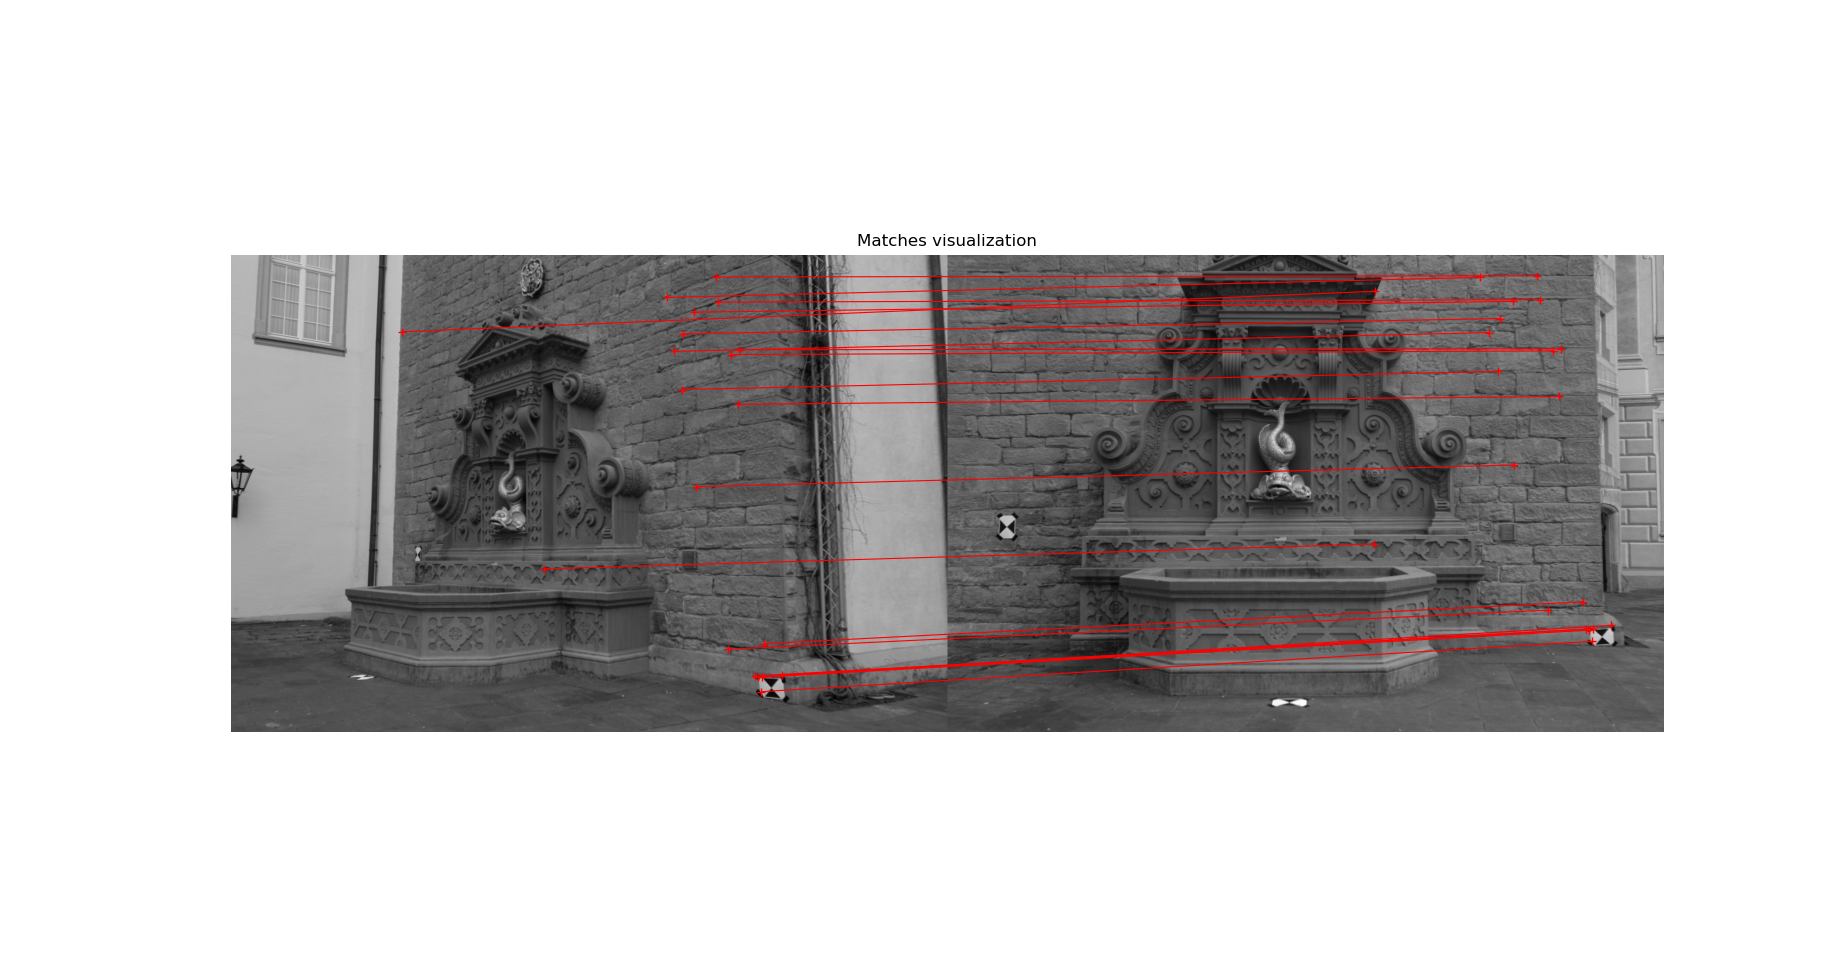
\includegraphics[width=1.0\linewidth]{putative_matches.png}
%     \caption{Putative matches after passing Lowe's ratio test.}
%     \label{fig:putative_matches}
% \end{figure}


% ========== Edit your name here
\author{Due by 11:59pm Friday, Mar 25th 2022}
\title{CS 498: Assignment 3: Iterative Closest Point and Odometry}
\date{March 4, 2022}
\maketitle

\medskip


\section*{Submission}
In this assignment, you will code your own point cloud alignment and depth odometry algorithm to estimate camera poses and build 3D maps of the environment through raw depth observation. The starter code consists of 2 python files you will modify along with a folder of some images and metadata. Please put together a single PDF with your answers and figures for each problem, and submit it to Gradescope (Course Code: JBXJVZ). If your code produces figures, they should go in this pdf, along with a description of what you did to solve the problem. We recommend you add your answers to the latex template files we provided. For code submission, make sure you use the provided ".py" files with your modification and the dumped ``.npz'' file. The graders will check both your PDF submission and your code submission if needed. 

\section*{Iterative Closed Point} 

In this part, your task is to align two point clouds. The algorithm we will leverage is called the iterative closed point. There are several components. 

\paragraph{Question 1 (Unprojection)[1 pts]:} Here, you will be modifying the function "rgbd2pts" in "icp.py". Given the input RGB-D image and the intrinsic matrix, your task is to unproject the RGB-depth image observations back to 3D as a form of a colored point cloud. We provide an open3d visualization for the point cloud and you should report the resulting figure in the document. Meanwhile, please avoid solutions using for-loop or directly calling off-the-shelf unprojection function.
\paragraph{Answer:} 
\begin{quote}

Below is the implentation of RGB-D projection onto the 3-D space:

\begin{lstlisting}[language=Python, basicstyle=\scriptsize]
def rgbd2pts(color_im, depth_im, K):
    # Question 1: unproject rgbd to color point cloud, 
    # provide visualization in your document
    # Your implementation between the lines
    # ---------------------------
  
    # read image size 
    h, w = depth_im.shape 
    # read camera intrinsics
    f = np.linalg.norm(np.diag(K)[:-1])
    px, py = K[0:2,2]
  
    # convert depth data into 3d coordinate
    U, V = np.meshgrid(np.arange(w)-int(px), np.arange(h)-int(py))
    X = U * depth_im / f
    Y = V * depth_im / f
    
    # create 3d pointcloud and color data
    xyz = np.stack([X,Y,depth_im], axis=2)
    xyz = xyz.reshape((-1,3))
    color = color_im.reshape((-1,3))
    
    # ---------------------------
    
    pcd = o3d.geometry.PointCloud()
    pcd.points = o3d.utility.Vector3dVector(xyz)
    pcd.colors = o3d.utility.Vector3dVector(color)
    return pcd
\end{lstlisting}

Beware that the mapping from the RGB-D to the 3-D space is governed by the widely adapted camera projection model; the ratio of the focal length to the depth is proportional to that of the 2D image to the 3D space coordinate. 

For a sanity check, the visualization of the raw source and the target pointclouds are shown in Fig.~\ref{fig:pcds_raw}. It is confirmed that the \texttt{rgbd2pts} function is well-designed without causing any glitch.

\begin{figure}[h]
    \centering
    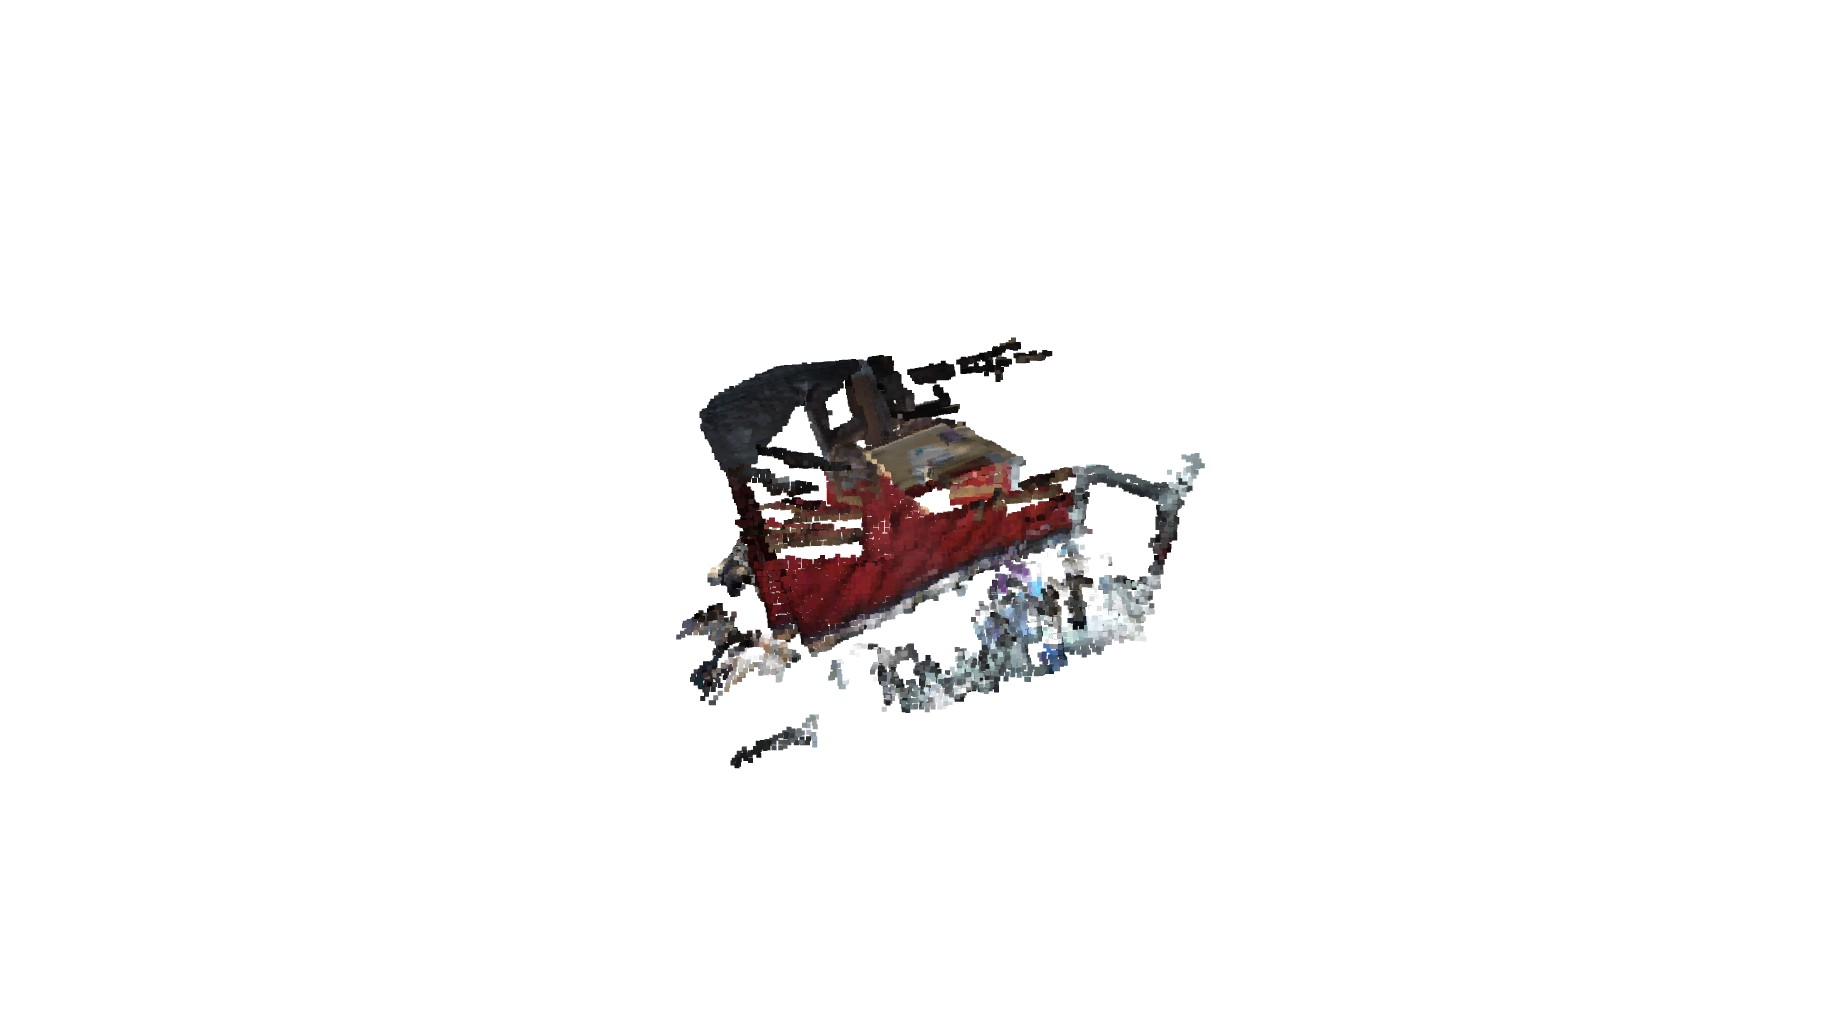
\includegraphics[width=1.0\linewidth]{pcds_raw.jpg}
    \caption{Source and target pointclouds before alignment.}
    \label{fig:pcds_raw}
\end{figure}

\end{quote}

\paragraph{Question 2 (Rigid Transform Fitting) [3 pts]:} Here, you will be modifying the function "fit\_rigid" in "icp.py". For this question, your task is to implement the rigid transformation fitting algorithm, assuming you are given N pairs of corresponding 3d points. You should refer to our lecture slide on depth sensing, and additional references could be found here: \href{https://www.ltu.se/cms_fs/1.51590!/svd-fitting.pdf}{link1}, \href{https://igl.ethz.ch/projects/ARAP/svd_rot.pdf}{link2}, \href{https://en.wikipedia.org/wiki/Orthogonal_Procrustes_problem}{link3}. You will use the point-to-point distance in this part. 
In addition, please provide an answer and necessary mathematical justification on what will happen if the input corresponding point pair contains errors and whether you could identify such situation. % \textbf{TODO: Do you mean whether they could identify such errors?}. 
\paragraph{Answer:} 
\begin{quote}

Below is the implentation of rigid transform fitting:

\begin{lstlisting}[language=Python, basicstyle=\scriptsize]
def fit_rigid(src, tgt, point_to_plane=False, src_normal=None):
    # Question 2: Rigid Transform Fitting
    # Implement this function
    # -------------------------
  
    assert len(src) == len(tgt)
  
    T = np.identity(4)
    
    # point-to-point algorithm
    # https://igl.ethz.ch/projects/ARAP/svd_rot.pdf
    if not point_to_plane:
      # assume that weights are equal
      # calculate centroid
      src_avg = np.mean(src, axis=0)
      tgt_avg = np.mean(tgt, axis=0)
      
      # construct 3x3 covariance matrix
      C = (src - src_avg).T @ (tgt - tgt_avg)
      
      # do svd 
      U, S, Vh = np.linalg.svd(C)
      
      # reconstruct rotation matrix
      M = np.eye(3)
      M[2,2] = np.linalg.det(Vh.T @ U.T)
      
      R = Vh.T @ M @ U.T
  
      # reconstruct translation matrix
      t = tgt_avg - R @ src_avg
      
      # write on SE(3) matrix
      T[:3,:3] = R
      T[:3,-1] = t
    
    ...
    
    return T
\end{lstlisting}

The overall logic comes from [\href{https://igl.ethz.ch/projects/ARAP/svd_rot.pdf}{here}]. Given corresponding pairs of pointcloud date, the rotation matrix is calculated by SVD first. Then, the translation between two sets of pointclouds is obtained from the aforementioned rotation matrix estimate and the their centroids. In conclusion, the $SE(3)$ matrix transforming the coordinate from that of \texttt{src} to that of \texttt{tgt} is returned.

\color{red}
%% TODO: FILL HERE
In addition, please provide an answer and necessary mathematical justification on what will happen if the input corresponding point pair contains errors and whether you could identify such situation.

\begin{itemize}
    \item 
\end{itemize}

\end{quote}

\paragraph{Question 3 (Point-to-Point ICP Loop) [3 pts]:} Here you will be modifying the function "icp" in "icp.py". Your task is to complete the full ICP algorithm. You are provided a starter code with hints in the comments. Please complete it and try to align the provided two point clouds. We provide a visualization for the aligned results which includes your estimated camera poses compared to the GT camera poses. Please provide an image of the final visualization in this pdf along with a description of the algorithm.
\paragraph{Answer:} 
\begin{quote}

Below is the implentation of iterative closest point algorithm:

\begin{lstlisting}[language=Python, basicstyle=\scriptsize]
def icp(source, target, max_iter=20, point_to_plane=False, inlier_thres=0.1):
  # Question 3: ICP
  # Hint 1: using KDTree for fast nearest neighbour
  # Hint 3: you should be calling fit_rigid inside the loop
  # You implementation between the lines
  # ---------------------------------------------------
  T = np.eye(4)     # initial guess of transformation matrix 
  transforms = []   # total transformation after every iteration
  delta_Ts = []     # incremental transformation for every iteration

  inlier_ratio = 0
  print("iter %d: inlier ratio: %.2f" % (0, inlier_ratio))

  for i in range(max_iter):
    # construct kd tree
    tree = KDTree(src)
    # find corresponding pairs (the nearest)
    dist, idx = tree.query(tgt, k=1)
    dist = dist.flatten(); idx = idx.flatten()
    # count inlier ratio
    inlier_ratio = len(np.where(dist < inlier_thres)[0]) / len(tgt)

    # find incremental transformation matrix
    T_delta = fit_rigid(src[idx], tgt, point_to_plane=point_to_plane, \
                        src_normal=src_normal[idx])
    # update total transformation matrix
    T = T_delta @ T
    # update src points
    src = (T_delta @ np.c_[src, np.ones(len(src))].T)[:3, :].T

    # ---------------------------------------------------
  ...
  return transforms, delta_Ts
\end{lstlisting}

The basic logic follows the intruction. First, the nearest points in \texttt{src} to the points in \texttt{tgt} is found by the off-the-shelf KD tree and search algorithm. Then, the \texttt{fit\_rigid} is executed with the candidates of those nearest pairs. As a result, the incremental update of transformation matrix \texttt{T\_delta} is obtained. This matrix is used to update both the accumulated $SE(3)$ transformation matrix from the \texttt{src} to the \texttt{tgt} and the pointcloud \texttt{src} until the maximum iteration or the covergence fulfilling the inlier threshold. 

The final aligned source and target pointclouds upon the point-to-point ICP algorithm are shown in Fig.~\ref{fig:pcds_icp_point2point}.
\begin{figure}[h]
    \centering
    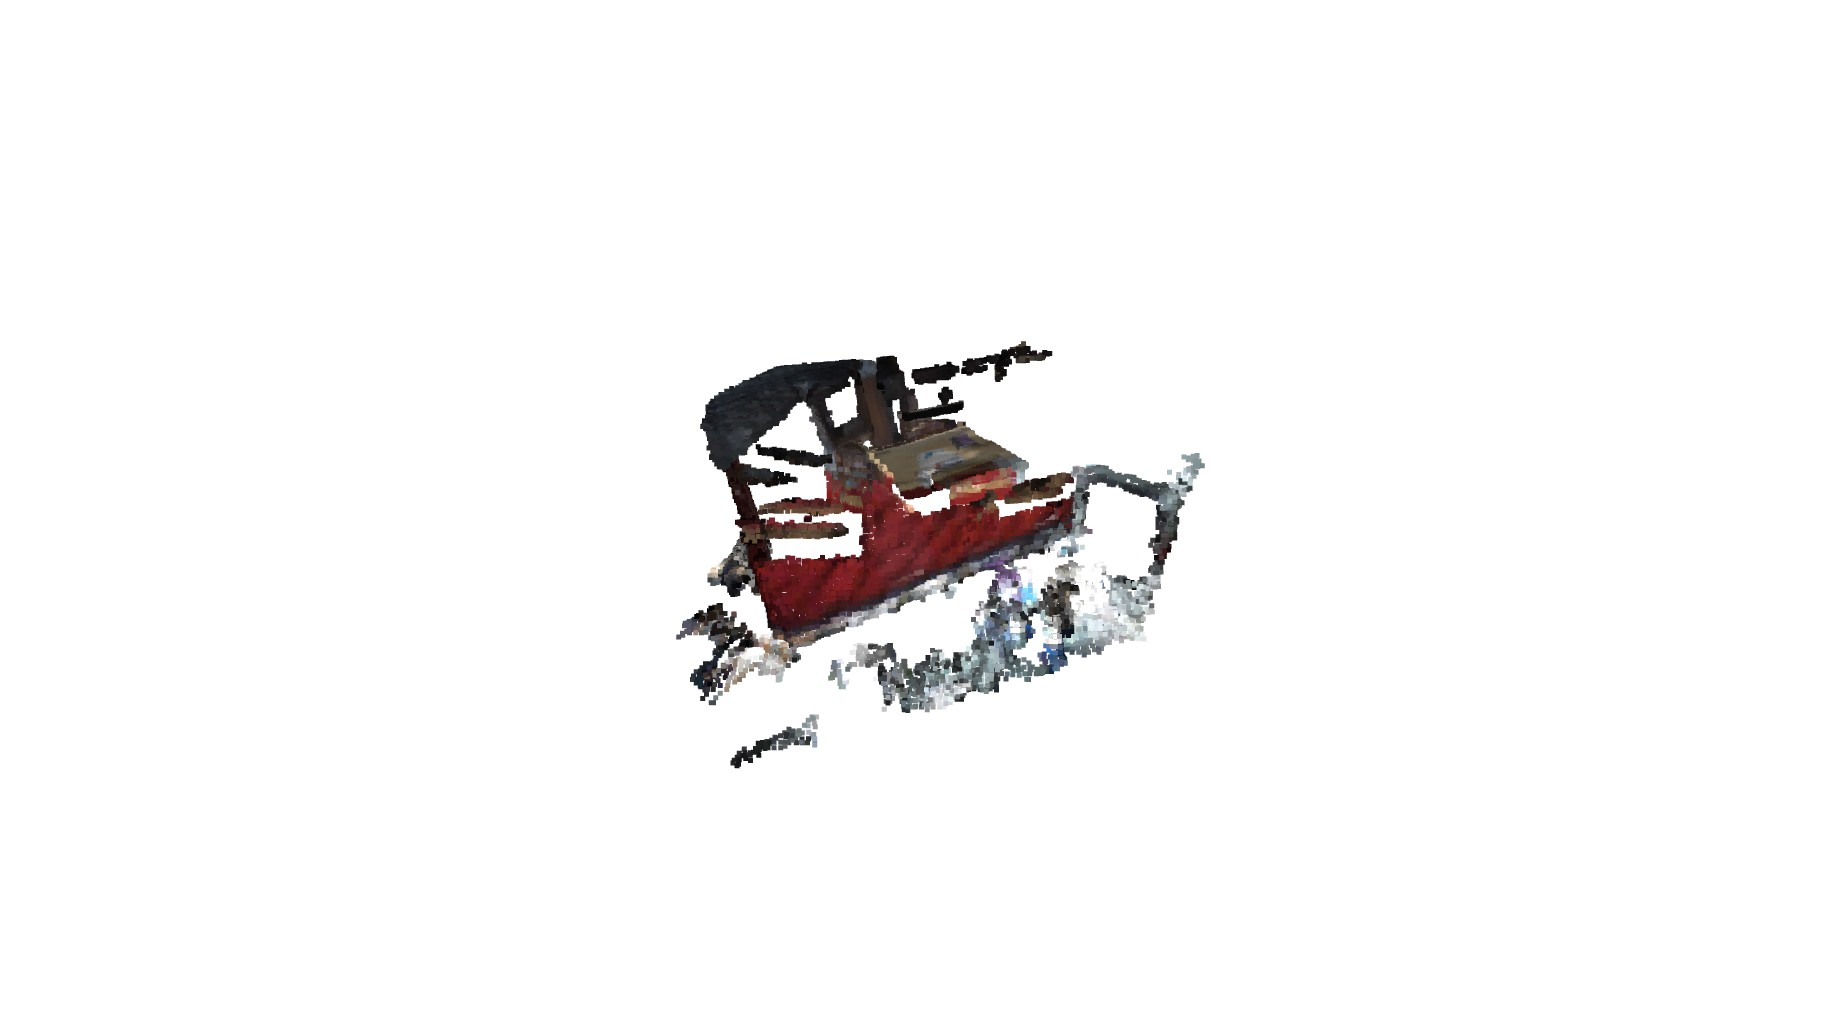
\includegraphics[width=1.0\linewidth]{pcds_icp_point2point.jpg}
    \caption{Aligned source and target pointclouds after running the point-to-point ICP.}
    \label{fig:pcds_icp_point2point}
\end{figure}

\end{quote}


\paragraph{Question 4 (Point-to-Plane ICP) [2 pt]:} Here you will be modifying "icp.py". Please extend your point-to-point ICP to allow it to take point-to-plane distance. Please run the alignment on your testing cases again and visualize the alignment results. Please justify when point-to-plane might be preferred over point-to-point distances (provide mathematical justification if necessary). 
\paragraph{Answer:} 
\begin{quote}

Point-to-plane ICP can be executed by setting the parameter \texttt{point\_to\_plane} of the function \texttt{icp} to be true. For instance:

\begin{lstlisting}[language=Python, basicstyle=\scriptsize]
icp(source, target, max_iter=20, point_to_plane=True, inlier_thres=0.1)
\end{lstlisting}

The only difference happens inside the function \texttt{icp}, by calling the function \texttt{fit\_rigid} with the argument \texttt{point\_to\_plane=True}. Below illustrates how the function \texttt{fit\_rigid(point\_to\_plane=True)} works:

% point-to-plane fitting function
\begin{lstlisting}[language=Python, basicstyle=\scriptsize]
def fit_rigid(src, tgt, point_to_plane=True, src_normal=None):
  # point-to-point algorithm
  # https://igl.ethz.ch/projects/ARAP/svd_rot.pdf
  if not point_to_plane:
    ...
  # point-to-plane algorithm
  # https://www.cs.princeton.edu/~smr/papers/icpstability.pdf
  else:
    A = np.empty((6*len(src), 6))
    b = np.empty(6*len(src))

    # construct overdetermined linear system
    for i, (p,q,n) in enumerate(zip(src,tgt,src_normal)):
      c = np.cross(p,n)
      v = np.concatenate([c,n])
      A[6*i:6*(i+1)] = np.outer(v,v)
      b[6*i:6*(i+1)] = - v * np.inner(p-q, n)
    
    # get solution to the overdetermined system
    x = np.linalg.lstsq(A, b, rcond=None)[0]

    # recover translation
    t = x[3:]

    # recover rotation
    a, b, c = x[:3]
    R = np.array([[1,-c,b],
                  [c,1,-a],
                  [-b,a,1]])
    from scipy.spatial.transform import Rotation
    rot = Rotation.from_matrix(R)
    R = Rotation.as_matrix(rot)

    # write on SE(3) matrix
    T[:3,:3] = R
    T[:3,-1] = t
  
  # -------------------------
  return T
\end{lstlisting}

The basic algorithm comes from [\href{https://www.cs.princeton.edu/~smr/papers/icpstability.pdf}{here}]; unlike point-to-point ICP, the translation and rotation is obtained simultaneously by solving a least-square problem as formulated in the aforementioned paper. In conclusion, the $SE(3)$ matrix transforming the coordinate from that of \texttt{src} to that of \texttt{tgt} is returned.

The final aligned source and target pointclouds upon the point-to-plane ICP algorithm are shown in Fig.~\ref{fig:pcds_icp_point2plane}.
\begin{figure}[h]
    \centering
    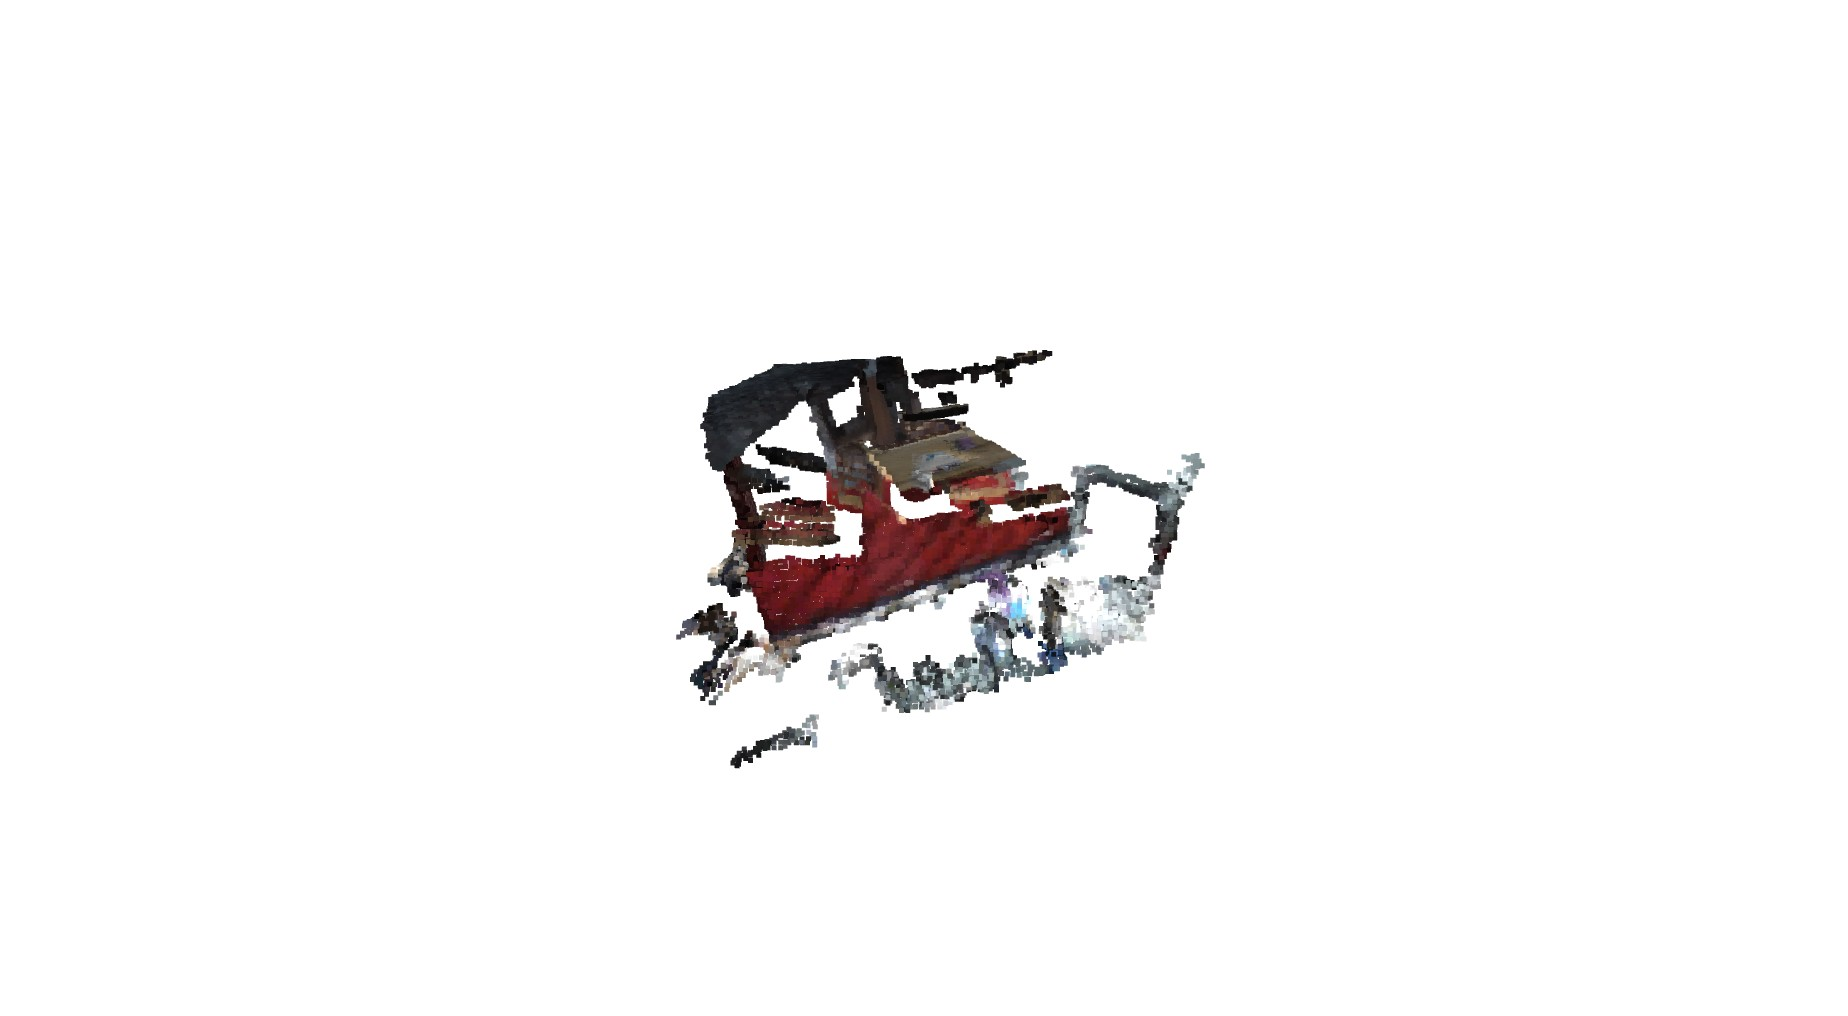
\includegraphics[width=1.0\linewidth]{pcds_icp_point2plane.jpg}
    \caption{Aligned source and target pointclouds after running the point-to-plane ICP.}
    \label{fig:pcds_icp_point2plane}
\end{figure}

\color{red}
%% TODO: FILL HERE

Please justify when point-to-plane might be preferred over point-to-point distances (provide mathematical justification if necessary).

\begin{itemize}
    \item 
\end{itemize}

\end{quote}


\paragraph{Question 5 (Translation and Rotation Error) [1 pt]:} Now, we would like to evaluate how good our estimated poses are. Unlike other prediction tasks where the output is categorical data or euclidean vectors, pose estimation lies in SE(3) space. And we might want to evaluate rotation and translation components separately. Please check this reference and implement the translation and rotation error defined in Eq. 5-6. (\href{https://cmp.felk.cvut.cz/~hodanto2/data/hodan2016evaluation.pdf}{link}). Please report your translation and rotation errors for the two ICP algorithms, along with the estimated and gt pose.  
\paragraph{Answer:} 
\begin{quote}

Below is the implentation of translation and rotation error as introduced [\href{https://cmp.felk.cvut.cz/~hodanto2/data/hodan2016evaluation.pdf}{here}]:

\begin{lstlisting}[language=Python, basicstyle=\scriptsize]
def pose_error(estimated_pose, gt_pose):
    # Question 5: Translation and Rotation Error 
    # Use equations 5-6 in https://cmp.felk.cvut.cz/~hodanto2/data/hodan2016evaluation.pdf
    # Your implementation between the lines
    # ---------------------------
    error = 0
  
    error_trn = np.linalg.norm(estimated_pose[:3, -1] - gt_pose[:3, -1])
    error_rot = np.arccos((np.trace(estimated_pose[:3,:3] @ gt_pose[:3,:3].T) - 1) / 2)
    
    print(f" -- translation error: {error_trn:.2f} [m]")
    print(f" -- rotation error   : {np.rad2deg(error_rot):.2f} [deg]")
    
    error = (error_trn, error_rot)
    # ---------------------------
    return error
\end{lstlisting}

Here, we report the translation and rotation error of running the point-to-point ICP, along with its estimate and ground-truth.

% point-to-point ICP (1. error 2. gt and estimated pose)
{\tt
-- translation error: 0.0975 [m]    \\
-- rotation error   : 3.5062 [deg]  \\
Ground truth pose:  
[[ 0.9983 -0.0386  0.043   0.0579]
[ 0.0402  0.9985 -0.038   0.0361] 
[-0.0415  0.0397  0.9984 -0.0679] 
[ 0.      0.      0.      1.    ]] \\
Estimated pose:
[[ 0.9983  0.021   0.0546 -0.0335]
[-0.0192  0.9993 -0.0324  0.0448]
[-0.0553  0.0313  0.998  -0.1008]
[ 0.      0.      0.      1.    ]]
}

Here, we report the translation and rotation error of running the point-to-plane ICP, along with its estimate and ground-truth.

% point-to-plane ICP (1. error 2. gt and estimated pose)
{\tt
-- translation error: 0.1247 [m]    \\
-- rotation error   : 2.0591 [deg]  \\
Ground truth pose:
[[ 0.9983 -0.0386  0.043   0.0579]
[ 0.0402  0.9985 -0.038   0.0361] 
[-0.0415  0.0397  0.9984 -0.0679] 
[ 0.      0.      0.      1.    ]]  \\
Estimated pose:
[[ 0.9971 -0.0381  0.066  -0.058 ]
[ 0.0389  0.9992 -0.0102  0.0137] 
[-0.0656  0.0128  0.9978 -0.108 ] 
[ 0.      0.      0.      1.    ]]
}

It is observed that both ICP algorithms shows the translation error about an negative order of magnitude. The point-to-plane ICP demonstrates the better rotational error by 1 degree compared with the point-to-point ICP.

\end{quote}

\pagebreak

\section*{Odometry} 
Now we will expand to estimate the trajectory of camera poses from an RGBD image sequence.

\paragraph{Question 6 (Odometry) [2 pts]:}
Here you will be modifying "odometry.py". Your task is to estimate the camera pose in an incremental fashion, which means that we will estimate camera pose $\mathbf{T}_t$ assuming the previous step's camera pose $\mathbf{T}_{t-1}$ is given. The key is to leverage ICP and estimate the relative transformation between the two and apply the difference through pose composition to get the current step's estimation. We will assume that frame 0's camera coordinate is the world frame origin. We also provide helper functions to visualize the aligned point cloud, read the GT camera poses and visualize the camera trajectory. Please complete the provided code and report the point cloud alignment and camera trajectory in your report. 
\paragraph{Answer:} 
\begin{quote}

Below is the algorithm of an RGB-D odometry based on ICP for every consecutive frame.

\begin{lstlisting}[language=Python, basicstyle=\small]
# incremental pose difference
final_Ts, _ = icp(source_down, target_down, inlier_thres=0.01)
T_inc =  final_Ts[-1]
# update latest camera pose wrt world frame
T_W2C = np.linalg.inv(T_inc) @ T_W2C

pred_poses[frame] = T_W2C
\end{lstlisting}

If a new $i+1$th frame is given, the $SE(3)$ transformation matrix \texttt{T\_inc} representing the transformation from the $i$th to the $i+1$th frame ($^{i+1}_{i}\mathbf{T}$) is yielded by calling the \texttt{icp} function. Its inverse is then left-multiplied to the matrix \texttt{T\_W2C}, which denotes the transformation from the $i$th frame to the world frame; hence, the $i$th camera pose with resepect to the world frame. As a result, a new updated camera pose at $i+1$th timestep is obtained, as $^{W}_{i+1}\mathbf{T} = ^{i}_{i+1}\mathbf{T} ~ ^{W}_{i}\mathbf{T}$. This workflow is iteratively executed for every input frame and hence, the estimate of camera trajectory can be obtained, as reported in Fig.~\ref{fig:gt_odom}.

\begin{figure}[h]
    \centering
    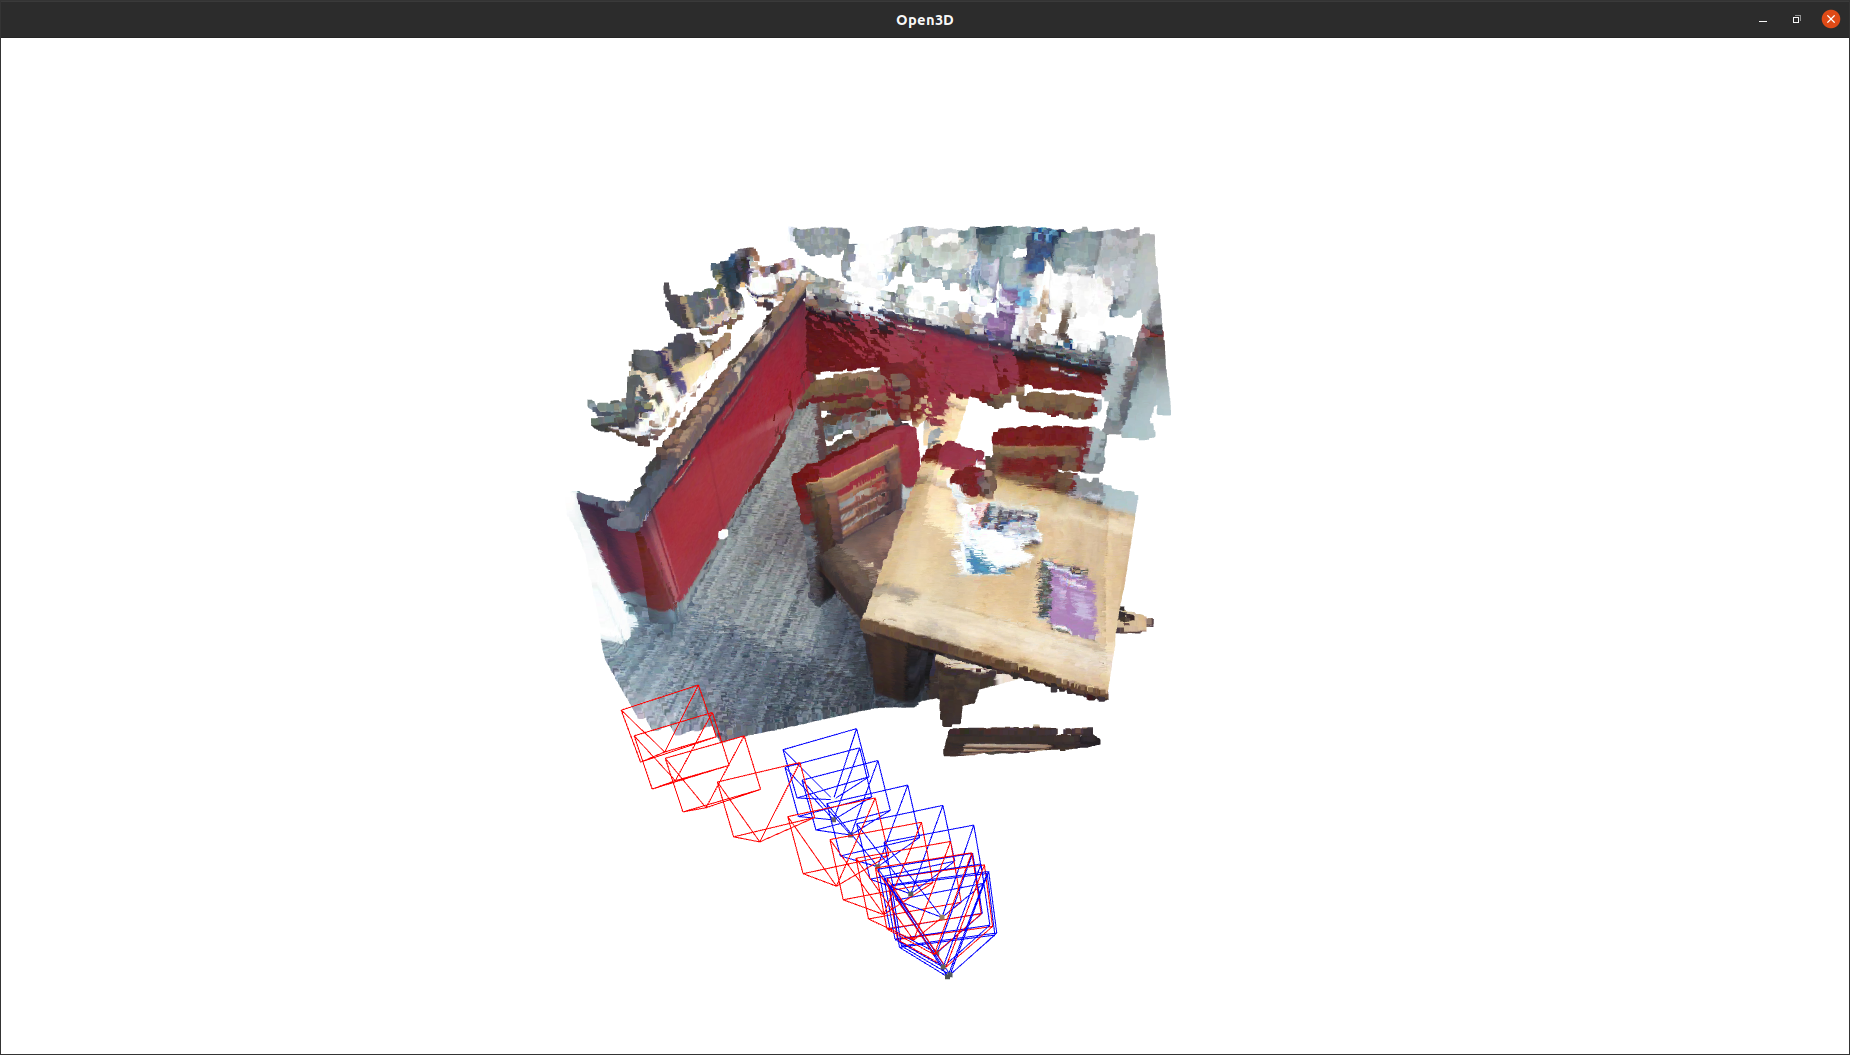
\includegraphics[width=1.0\linewidth]{gt_odom.png}
    \caption{Trajectory estimates from odometry (blue) and its ground truth (red).}
    \label{fig:gt_odom}
\end{figure}

\end{quote}


\paragraph{Question 7 (Relative Trajectory Error) [2 pts]:}
Odometry cares about the accuracy of the relative poses. Due to the global pose drift, estimating the absolute pose error as we did for ICP might not be suitable for evaluating odometry. Thus, people use average relative pose error to measure the pose estimation accuracy for odometry/slam algorithms. Based on your implemented rotation and translation error estimation algorithm, please implement the following average relative pose error: (\href{http://www.cvlibs.net/publications/Geiger2012CVPR.pdf}{link} eq. 2 and eq. 3). Please visualize the estimated trajectory and ground-truth trajectory and report the error. 
% \textbf{TODO: What should they put in pdf}
\paragraph{Answer:} 
\begin{quote}

Below is the implementation of calculating the relative trajectory error for consecutive frames, as denoted in Eq.~(2) and Eq.~(3) of [\href{http://www.cvlibs.net/publications/Geiger2012CVPR.pdf}{here}]. 

\begin{lstlisting}[language=Python, basicstyle=\scriptsize]
## function calculating relative trajectory error framewise
def get_rte(pred_poses, gt_poses):
  from scipy.spatial.transform import Rotation
  assert len(pred_poses) == len(gt_poses)

  rte_rot = 0
  rte_trn = 0

  for frame in range(step, end, step):
    delT_pred = pred_poses[frame] @ np.linalg.inv(pred_poses[frame-step])
    delT_gt = gt_poses[frame] @ np.linalg.inv(gt_poses[frame-step])
    delT_pred_gt = delT_pred @ np.linalg.inv(delT_gt)
    
    t = delT_pred_gt[:3,-1]
    R = delT_pred_gt[:3,:3]
    rot = Rotation.from_matrix(R)
    
    rte_rot += rot.magnitude()
    rte_trn += np.linalg.norm(t)

  rte_rot /= (len(gt_poses)-1)
  rte_trn /= (len(gt_poses)-1)

  print(f" -- RTE (translation): {rte_trn:.2f} [m]  ")
  print(f" -- RTE (rotation)   : {np.rad2deg(rte_rot):.2f} [deg]")

  return rte_trn, rte_rot

## report RTE of the aforementioned odometry result
get_rte(pred_poses, gt_poses)
\end{lstlisting}

We report the average relative trajectory error for every consecutive frames. Again, the estimated trajectory and its ground truth are illustrated in Fig.~\ref{fig:gt_odom}.

{\tt
-- RTE of odometry:                 \\
-- RTE (translation): 0.03 [m]      \\
-- RTE (rotation)   : 0.94 [deg]    
}

\end{quote}

\paragraph{Question 8 (Pose Graph Optimization) [2 pts]:}
So far, we have been only leveraging the relative transformation between adjacent frames. Absolute poses in global space are computed by accumulating the relative transformations. Do you think it is the best idea? What if there is one pair with a catastrophic alignment error? Given the odometry pose estimation of frame 0 and frame 40, % \textbf{TODO: in code it is 0 and 40} 
% pose estimation, 
do you anticipate that they will be consistent with directly running ICP estimation between their corresponding point cloud? In this question, you will leverage a tool called pose graph optimization to help with the challenge. The general idea is simple: each frame's pose is a node in this graph, and any frames could be connected through an edge. On each edge, we define a cost measuring the agreement between the relative pose estimate between the two nodes and their pose estimation. By minimizing the energy, we are promoting global consistency across all the frames. More guidance is provided in the code.
\paragraph{Answer:} 
\begin{quote}

Below is the implementation of the odometry leveraging graph optimization up to three adjacent frames.

\begin{lstlisting}[language=Python, basicstyle=\scriptsize]
# initialize graph to be optimized
pose_graph = o3d.pipelines.registration.PoseGraph()
frame_list = list(pred_poses.keys())

voxel_size=0.02
max_correspondence_distance_coarse = voxel_size * 15
max_correspondence_distance_fine = voxel_size * 1.5

...

# add all nodes
for frame_id in frame_list:
  T_i2W = np.linalg.inv(pred_poses[frame_id])
  pose_graph.nodes.append(o3d.pipelines.registration.PoseGraphNode(T_i2W))

# add all edges
for i, src_id in enumerate(frame_list):
  for k in range(1,4):
    if i+k < len(frame_list):
      tgt_id = frame_list[i+k]
      print(f' -- add edge from {src_id} to {tgt_id} ... ')
      # run icp between frame i and j (i+k)
      final_Ts, _ = icp(pcds[src_id], pcds[tgt_id], inlier_thres=0.01)
      T_i2j =  final_Ts[-1]
      # add an edge
      pose_graph.edges.append(o3d.pipelines.registration.PoseGraphEdge(i, i+k, T_i2j))

...
# run optimization
print("Optimizing PoseGraph ...")

option = o3d.pipelines.registration.GlobalOptimizationOption(
    max_correspondence_distance=max_correspondence_distance_fine,
    edge_prune_threshold=0.25,
    reference_node=0)
with o3d.utility.VerbosityContextManager(o3d.utility.VerbosityLevel.Debug) as cm:
    o3d.pipelines.registration.global_optimization(
        pose_graph,
        o3d.pipelines.registration.GlobalOptimizationLevenbergMarquardt(),
        o3d.pipelines.registration.GlobalOptimizationConvergenceCriteria(),
        option)

\end{lstlisting}

We report the average relative trajectory error (1) from the odometry and (2) from the graph optimization.

{\tt
-- RTE of odometry:                 \\
-- RTE (translation): 0.03 [m]      \\
-- RTE (rotation)   : 0.94 [deg]    
}

{\tt
-- RTE of graph optimization:       \\
-- RTE (translation): 0.02 [m]      \\
-- RTE (rotation)   : 0.59 [deg]
}

It is shown that the result from graph optimization yields smaller error by 0.01~\textrm{m} for translation and 0.35~\textrm{deg} for rotation. Also, as shown in Fig.~\ref{fig:gt_odom_opt}, the odometry with graph optimization get close to the ground truth trajectory.

\begin{figure}[h]
    \centering
    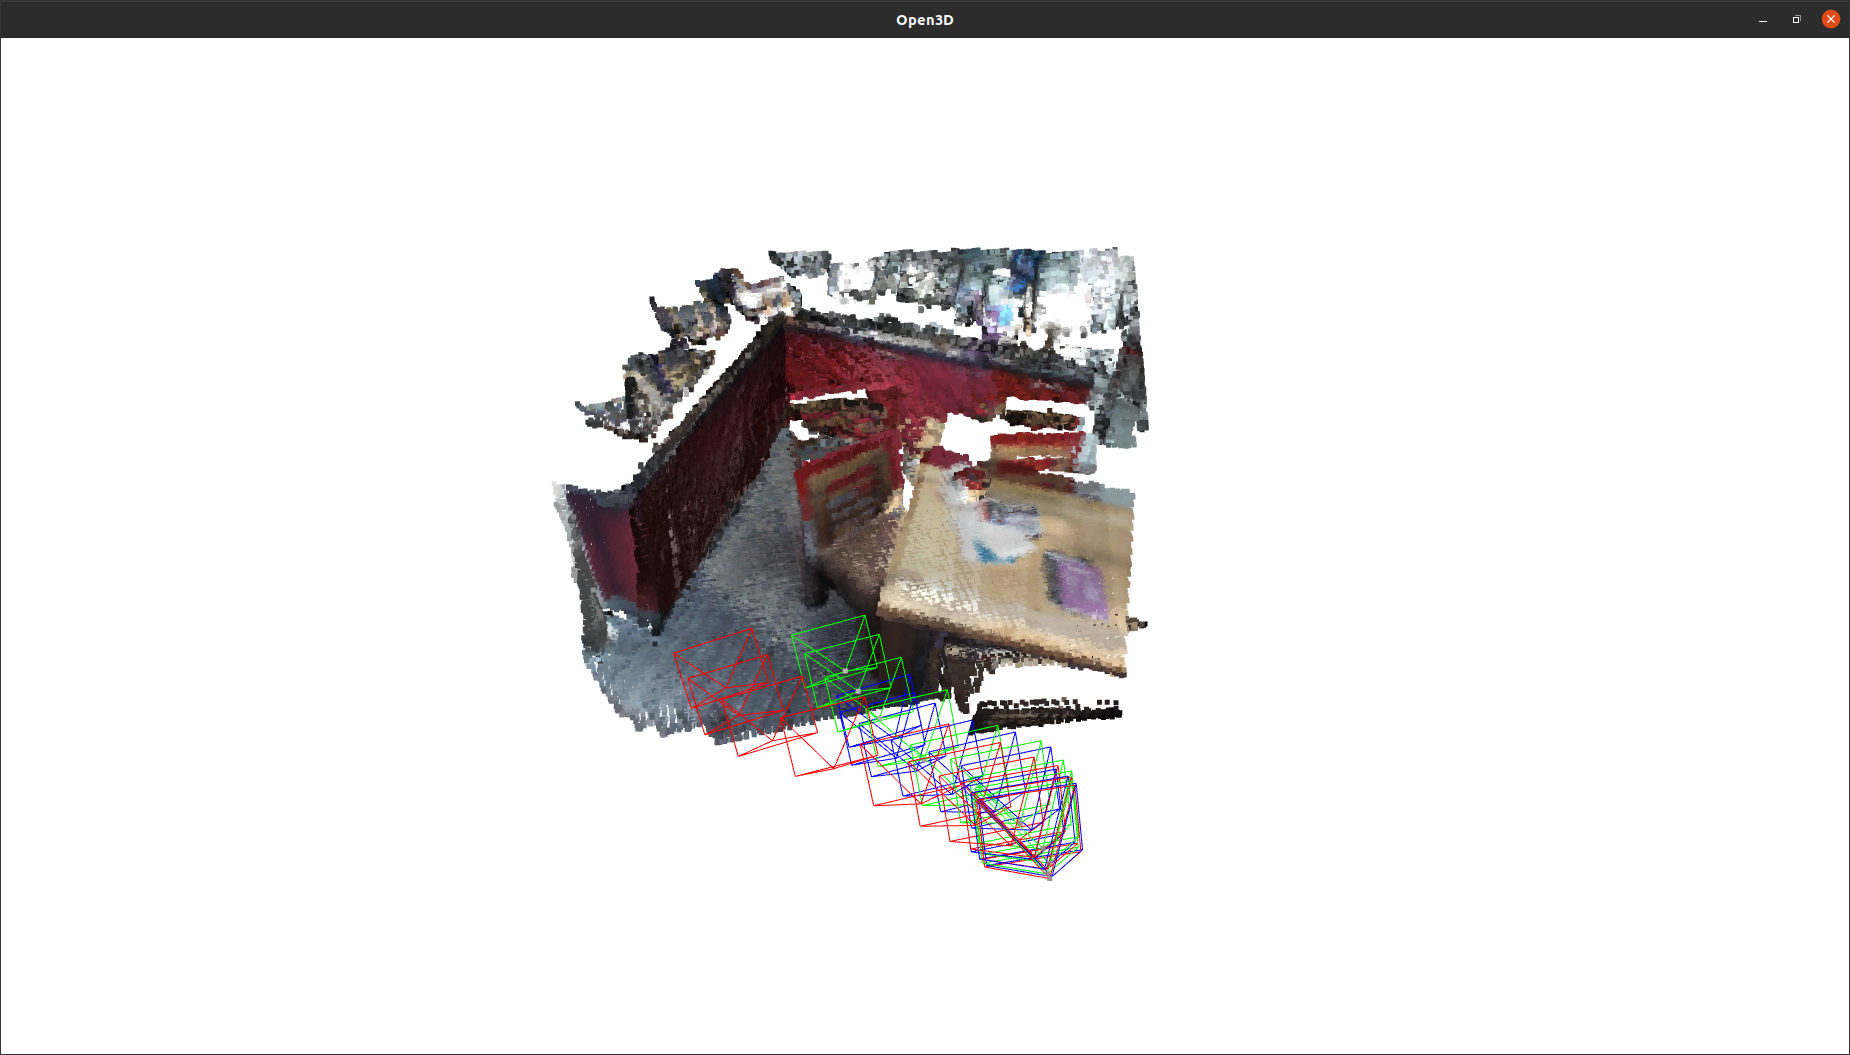
\includegraphics[width=1.0\linewidth]{gt_odom_opt.png}
    \caption{Trajectory estimates from odometry (blue) and from graph optimization (green) compared to the ground truth (red).}
    \label{fig:gt_odom_opt}
\end{figure}

\end{quote}


\section*{Mapping (Bonus 3pt)}

We believe you have a great camera trajectory estimation now. This bonus question will leverage the well-aligned camera trajectory and build a 3D map of the room. The general idea is to leverage volumetric fusion, described in KinectFusion paper and covered in our lecture. The key is to incrementally update the signed distance values for each voxel in the volume if a new depth frame comes. Try to fuse the color and depth into the volume and use a marching cube to get the extracted mesh. Leveraging existing volumetric fusion functions will not count. That being said, you could use them as a sanity check. You are allowed to use the GT camera poses. Try your best to get visually appealing results. We will choose the top solution and announce them in the class. 
\end{document}. 

\grid
\grid